
% Template for Elsevier CRC journal article
% version 1.2 dated 09 May 2011

% This file (c) 2009-2011 Elsevier Ltd.  Modifications may be freely made,
% provided the edited file is saved under a different name

% This file contains modifications for Energy Procedia

% Changes since version 1.1
% - added "procedia" option compliant with ecrc.sty version 1.2a
%   (makes the layout approximately the same as the Word CRC template)
% - added example for generating copyright line in abstract

%-----------------------------------------------------------------------------------

%% This template uses the elsarticle.cls document class and the extension package ecrc.sty
%% For full documentation on usage of elsarticle.cls, consult the documentation "elsdoc.pdf"
%% Further resources available at http://www.elsevier.com/latex

%-----------------------------------------------------------------------------------

%%%%%%%%%%%%%%%%%%%%%%%%%%%%%%%%%%%%%%%%%%%%%%%%%%%%%%%%%%%%%%
%%%%%%%%%%%%%%%%%%%%%%%%%%%%%%%%%%%%%%%%%%%%%%%%%%%%%%%%%%%%%%
%%                                                          %%
%% Important note on usage                                  %%
%% -----------------------                                  %%
%% This file should normally be compiled with PDFLaTeX      %%
%% Using standard LaTeX should work but may produce clashes %%
%%                                                          %%
%%%%%%%%%%%%%%%%%%%%%%%%%%%%%%%%%%%%%%%%%%%%%%%%%%%%%%%%%%%%%%
%%%%%%%%%%%%%%%%%%%%%%%%%%%%%%%%%%%%%%%%%%%%%%%%%%%%%%%%%%%%%%

%% The '3p' and 'times' class options of elsarticle are used for Elsevier CRC
%% The 'procedia' option causes ecrc to approximate to the Word template
\documentclass[3p,times,procedia]{elsarticle}

%% The `ecrc' package must be called to make the CRC functionality available
\usepackage{ecrc}

%% The ecrc package defines commands needed for running heads and logos.
%% For running heads, you can set the journal name, the volume, the starting page and the authors

%% set the volume if you know. Otherwise `00'
\volume{00}

%% set the starting page if not 1
\firstpage{1}

%% Give the name of the journal
\journalname{Energy Procedia}

%% Give the author list to appear in the running head
%% Example \runauth{C.V. Radhakrishnan et al.}
\runauth{}

\usepackage{multirow}


%% The choice of journal logo is determined by the \jid and \jnltitlelogo commands.
%% A user-supplied logo with the name <\jid>logo.pdf will be inserted if present.
%% e.g. if \jid{yspmi} the system will look for a file yspmilogo.pdf
%% Otherwise the content of \jnltitlelogo will be set between horizontal lines as a default logo

%% Give the abbreviation of the Journal.
\jid{egypro}

%% Give a short journal name for the dummy logo (if needed)
\jnltitlelogo{Energy Procedia}

%% Provide the copyright line to appear in the abstract
%% Usage:
%   \CopyrightLine[<text-before-year>]{<year>}{<restt-of-the-copyright-text>}
%   \CopyrightLine[Crown copyright]{2011}{Published by Elsevier Ltd.}
%   \CopyrightLine{2011}{Elsevier Ltd. All rights reserved}
\CopyrightLine{2011}{Published by Elsevier Ltd.}

%% Hereafter the template follows `elsarticle'.
%% For more details see the existing template files elsarticle-template-harv.tex and elsarticle-template-num.tex.

%% Elsevier CRC generally uses a numbered reference style
%% For this, the conventions of elsarticle-template-num.tex should be followed (included below)
%% If using BibTeX, use the style file elsarticle-num.bst

%% End of ecrc-specific commands
%%%%%%%%%%%%%%%%%%%%%%%%%%%%%%%%%%%%%%%%%%%%%%%%%%%%%%%%%%%%%%%%%%%%%%%%%%

%% The amssymb package provides various useful mathematical symbols
\usepackage{amssymb}
%% The amsthm package provides extended theorem environments
%% \usepackage{amsthm}

%% The lineno packages adds line numbers. Start line numbering with
%% \begin{linenumbers}, end it with \end{linenumbers}. Or switch it on
%% for the whole article with \linenumbers after \end{frontmatter}.
%% \usepackage{lineno}

%% natbib.sty is loaded by default. However, natbib options can be
%% provided with \biboptions{...} command. Following options are
%% valid:

%%   round  -  round parentheses are used (default)
%%   square -  square brackets are used   [option]
%%   curly  -  curly braces are used      {option}
%%   angle  -  angle brackets are used    <option>
%%   semicolon  -  multiple citations separated by semi-colon
%%   colon  - same as semicolon, an earlier confusion
%%   comma  -  separated by comma
%%   numbers-  selects numerical citations
%%   super  -  numerical citations as superscripts
%%   sort   -  sorts multiple citations according to order in ref. list
%%   sort&compress   -  like sort, but also compresses numerical citations
%%   compress - compresses without sorting
%%
%% \biboptions{comma,round}

% \biboptions{}

% if you have landscape tables
\usepackage[figuresright]{rotating}

% put your own definitions here:
%   \newcommand{\cZ}{\cal{Z}}
%   \newtheorem{def}{Definition}[section]
%   ...

% add words to TeX's hyphenation exception list
%\hyphenation{author another created financial paper re-commend-ed Post-Script}

% declarations for front matter
\usepackage{amsmath}
\usepackage{systeme}


\begin{document}

\begin{frontmatter}

%% Title, authors and addresses

%% use the tnoteref command within \title for footnotes;
%% use the tnotetext command for the associated footnote;
%% use the fnref command within \author or \address for footnotes;
%% use the fntext command for the associated footnote;
%% use the corref command within \author for corresponding author footnotes;
%% use the cortext command for the associated footnote;
%% use the ead command for the email address,
%% and the form \ead[url] for the home page:
%%
%% \title{Title\tnoteref{label1}}
%% \tnotetext[label1]{}
%% \author{Name\corref{cor1}\fnref{label2}}
%% \ead{email address}
%% \ead[url]{home page}
%% \fntext[label2]{}
%% \cortext[cor1]{}
%% \address{Address\fnref{label3}}
%% \fntext[label3]{}

\dochead{}
%% Use \dochead if there is an article header, e.g. \dochead{Short communication}
%% \dochead can also be used to include a conference title, if directed by the editors
%% e.g. \dochead{17th International Conference on Dynamical Processes in Excited States of Solids}

\title{Quantification of energy savings in smart buildings, physics or data?}


%% use optional labels to link authors explicitly to addresses:
%% \author[label1,label2]{<author name>}
%% \address[label1]{<address>}
%% \address[label2]{<address>}

\author{Aurora Gonz\'alez-Vidal}
\author{Alfonso Ramallo-Gonz\'alez}
%\author{Fernando Terroso-S\'aenz}
\author{Antonio F. Skarmeta}

\address{}

\begin{abstract}

Many efforts from several organisms are focused on the increasement of energy efficiency. It is on the interest of everybody, from particulars to governments, since energy efficiency yields to economical savings for households and companies, reduces greenhouse gas emissions benefiting environment, helps alleviate energy poverty and contributes to growth and jobs.
Before implementing an energy efficiency solution, it is neccesary to define the relationship which exists between energy use and the current operating conditions in order to determine energy savings that result form the implementation of the solution. 

Traditionally, white box models based on physics equations are used to model systems to predict whole buildings and their sub-systems behaviors, such as their energy consumption and indoor comfort. However, nowadays by means of the Internet of Things we count on vast amounts of data that can be used for knowledge extraction.

We propose a machine learning approach for the creation of an energy consumption prediction model that is used to estimate the energy consumption in normal operation state, i.e., if the  system would not have been altered by the energy efficiency experiment. This allows us to compare the predicted for normal operating state and the actual consumption in order to quantify the energy savings.

Our method shows better prediction accuracy than the so-called grey box methods.



\end{abstract}

\begin{keyword}
%% keywords here, in the form: keyword \sep keyword

%% PACS codes here, in the form: \PACS code \sep code

%% MSC codes here, in the form: \MSC code \sep code
%% or \MSC[2008] code \sep code (2000 is the default)

\end{keyword}

\end{frontmatter}


\section{Introduction}
\label{intro}

Energy consumption of buildings in developed countries comprises 20-40\% of total energy use and it is above industry and transport in EU and US \cite{perez2008review}. 

In order to adress climate change, together with the use of non-fossil and environmental friendly sources such as solar and wind, cutting energy consumption is also crucial. Reducing energy consumption to the necessary levels so as to keep comfort for buildings users helps to preserve finite resources and lowers the costs for consumers.

When it comes to energy savings, energy management is the process of monitoring, controlling, and conserving energy in a building. Typically this involves the following steps:

\begin{itemize}
\item Metering and collecting energy consumption data,
\item Proposing ways of saving energy by analysing the data and putting them into practice, and
\item Tracking the consumption in order to quantify the gains due to the proposed activity.
\end{itemize}

%We consider that there is a lack of variety in the way the third step is tackled nowadays. 

The collection of methods and processes used to face the third step, that is to asses the performance of energy efficiency activities by quantifying the gains on efficiency are called Evaluation, Measurement, and Verification (EM\&V). 

%In terms of the third step, the gains quantification is done through a collection of methods and processes used to assess the performance of energy efficiency activities called Evaluation, Measurement, and Verification (EM\&V). This has 

%The main objectives of an EM\&V process are to assess the performance of an energy efficiency program or project, to measure the energy or demand savings, and to determine if the program is generating the expected level of savings.

The traditional EM\&V methods for determine if a program is generating the expected level of savings are based on linear regression models and they are described in the ASHRAE’s Guideline \cite{ashrae2002ashrae}. 

Regression models need to be typically adjusted in ad hoc manners in order to capture nonlinear behavior, which arises from complex (physical) multivariable interactions between ambient conditions, occupancy levels, and building operating conditions \cite{heo2012gaussian}.

%[Expalin why we choose data analytics]

Regression has always been the standard approach to modeling the relationship between one outcome variable  and several input variables, and it can be seen both from a white-box and a black-box point of view. That means, we could use regression for analytical purposes, where a scenario is understood through physics or for data-driven purposes where a scenario is modeled using data alone. 

However, with recent advances in sensor and communication technologies, the generation of data about our surrounding environment and ourselves is explosively growing in terms of \emph{velocity}, \emph{variety} and \emph{volume}. This implies that there is more value hidden in the data and as the datasets are generally too large for a p-value to have meaning, predictive data-driven modeling uses other ways to fit a model such as machine learning.

%The other way to approach our problem is analytically, where models are often based on our understading of nature through physics. Those are called white-box models.

%https://ibm.cioreview.com/cxoinsight/the--black-box-paradox--in-big-data-analytics-and-datadriven-modeling-nid-18145-cid-117.html

%Analytical models are often based on a human’s understanding of nature, while data-driven and machine learning models attempt to model nature using data alone. Some data-driven models, such as linear regression, are transparent and interpretable, while other “black-box” models are not transparent and can be difficult to interpret.

Our proposal for evaluating the gains on energy consumption after an action implementation towards energy efficiency is to take a machine learning approach, where black box models are used in order to predict energy consumption, reducing the cost compared to traditional white box processes which require a level of building engineering expertise that limits scalability.




%\subsection{Regression vs Machine Learning}

%The Difference Between Predictive Modeling and Regression 

%when using predictive modeling, we can use many different models simultaneously, and compare  them to find the one that is the best. We can use the traditional regression, but also decision trees  and neural network analysis. We can also combine  different models. We can focus on accuracy of prediction rather than just i dentifying risk factors

%Regression requires an assumption of normality. The definition of confidence intervals, too, requires normality.

%Additional assumptions for regression are that the mean of the error term is equal to zero, and that the error term has equal variance for different levels of the input or independent variables. While the assumption of  zero mean is almost always satisfied, the assumpti on of equal variance is not

%With recent advances in sensor and communication technologies, the generation of data about our surrounding environment and ourselves is explosively growing in terms of \emph{velocity}, \emph{variety} and \emph{volume} \cite{ali2014}. The treatment of huge data sets challenges traditional technologies and promotes the emergence of \textbf{Big Data} tools in order to capture, store, manage and analyze such data. In this context, \textbf{Internet of Things (IoT)} is one of the key enablers of \textbf{Smart Cities}. We are part of a new \emph{Era} where sensing technologies are being exploited to create innovative services for Citizens and Service Providers.


%[Explain why daily and weekly is our interest]

\section{Related work}

Most of the building energy systems are complex nonlinear systems, which are strongly influenced by weather conditions, building operating modes, and occupant schedules.

Three general categories of building energy forecasting models have been reported in the literature which include white-box (physics-based), black-box (data-driven), and grey-box (combination of physics based and data-driven) modeling approaches \cite{li2014review}.

\subsection{White-box models}


Building structure, systems and equipments need to be considered for this kind of models together with weather conditions. The firsts are usually obtained from design plans, manufacture catalogues or need to be measured in place.

There exist a lot of mature white box simulation engines, that through the combination of mathematical equations simulate the building operation and calculate its energy consumption. Very well-known engines such as EnergyPlus \cite{crawley2001energyplus} and TRNSYS \cite{TRNSYS} have been widely used to analyze energy consumption and determine building control and operation scheme \cite{crawley2008contrasting}.

Even though these elaborate simulation tools are effective and accurate, they require detailed information and parameters of buildings, energy systems and outside weather conditions. These parameters, however, are always difficult to obtain, and sometimes they might not be available.

\subsection{Black-box models}


Black-box models are also known as solely data-driven model. In this case, statistical models are directly applied to capture the relationship between building energy consumption and the inputs: operation and weather data. This type of models need baseline measurements over a certain period of time.

Regression can be used as a data-driven model, however, it is highly more interpretable than machine learning approaches. 
Machine learning systems figure out how to solve problems with minimal human guidance and once a machine learning algorithm is trained, it can be difficult to understand why it gives a particular response to a set of data inputs. The adaptability of the machine learning models through a self-tuning process, which is different from mathematical models such as regression models, makes accurate decisions without outside expert intervention when unusual perturbations, disturbances, and/or changes in building background conditions occur.

Several data-based modeling techniques have been used for EM\&V, including multiple linear regression \cite{braun2014using},  Gaussian process modeling \cite{heo2012gaussian}.  %time series [4], 
In the case of machine learning techniques such as neural networks, support vector machines and their combination \cite{ahmad2014review} and fuzzy logic models \cite{ciabattoni2014fuzzy} are some examples.    

\subsection{Grey-box models}

Grey box models use simplified physical descriptions to simulate the behavior of building energy systems, and then identify important parameters and characteristics using statistical analysis \cite{handbook2017america}.
%Both statistical and machine learning methods need sufficient historical data to provide accurate models. 

Data-driven modelling based on grey-box models have been used for many years. As early of 1951 Burnard demonstrated for the first time that resistor-capacitor RC-networks can represent the thermodynamics of buildings accurately \cite{burnand1952study}. Since then, RC-networks have been used to represent the thermodynamics of buildings. In the early years of building dynamic simulation, this was one of the few ways of representing the thermodynamics of buildings, but even today, programs such as EnergyPlus, include thermal networks on their codes \cite{handbook2017america} .

In addition to building simulation, grey-box modelling of buildings using RC-networks have been used for the last two decades for Model Predictive Control (MDC). MDC has been used to govern heating and cooling systems of normally large buildings in a way in which the controller can anticipate to the needs of the building via the previous estimation of its thermodynamic features (these normally translated into response times and conductivity of the thermal envelope) \cite{coley1992second}.

In cases where limited amounts of data are available and the information about the building architecture is partially known, grey models are suitable alternatives for the prediction of electricity consumption \cite{hamzacebi2014forecasting}.



%A new approach to energy consumption prediction of domestic heat pump water heater based on grey system theory





%Artificial neural networks (ANN) is another popular method in building energy modeling for building operation purpose.

%predict cooling demand in a building. The energy demand was predicted using its measured or predicted values as well as the predicted values of air temperature and relative humidity \cite{yokoyama2009prediction}



\section{Methodology}

In this section we introduce both a black box and a grey box model based methodology in order to estimate the energy consumption of a building.

\subsection{Inputs}


Energy forecasting studies that use machine learning are usually intended to predict consumption a priori in order to manage and store the suitable amount of energy, taking into consideration the market prizes and also the necessities of the buildings. However, our approach is different in the sense that our goal is to quantify the energy savings relative to a baseline period due to certain experiment related to efficiency improvement. 
%evaluate a particular action that has been developed during a period of time and the prediction is done afterwards.

This translates into a difference in the inputs that are available for being used. In other scenarios, data concerning energy consumption in previous hours and days is very useful because it is evidently highly correlated with the later consumption \cite{aman2014empirical}. However, we should not use such data since the consumption is altered by the experiment.

On the other side, in other scenarios enviromental data is not available yet (it is the future) and predictions have to be used. When applying prediction for M\&V, environmental and occupation variables are usually available and it is not necesary to predict them. The most commonly used weather information is outdoor dry-bulb air temperature.


\subsection{Modeling}

Our interest lies on weekly quantification of the energy savings. However, daily dynamics are useful since there are patterns that can be found depending on the day of the week. In order to do so, we  predict daily energy consumption and then compute the metrics in a aggregated way so that the global quantification is done weekly.

\subsubsection{Black box approach}

Daily aggregate consumption is used as output and we try to capture the relationship between the whole day temperature and the consumption by relating the time series composed by every hours' mean temperature and the daily consumption.

Then, we can use several machine learning models in order to asses which is the best one for our scenarios. The models are generated  following the next steps \citep{gonzalez2016towards}:

\begin{itemize}
\item Clean and transform the data: selecting predictive variables such as temperature and day type, deleting outliers 
\item Aggregate: compute daily consumption, create the time series with the input variables and represent the series in a lower dimension. That is, apply hourly average or other representation and feature selection methods in order to serve as inputs of our models.
\item Divide the dataset into train (75 \% ) and test (25 \%)
\item Validation method: 10-fold cross validation and 5 repetitions over the training data set in order to find the hyperparameters of each machine learning algorithm
\item Evaluate: apply the algorithm to the test dataset in order to obtain the metric for the model
\end{itemize}


\subsubsection{ Grey box approach}


To make use of the models the set of outputs and inputs have to be defined together with the topology of the system. 
The most common mathematical representation of lumped parameter models is the state-space representation. The general form for time-invariant models can be written as shown on Eq. \ref{eq1}

\begin{equation}\label{eq1}
\systeme*{x'(t)=Ax(t) + Bu(t), y(t)= Cx(t) + Du(t)}
\end{equation}

where $x$ is a vector with the states of the model, in our case the temperatures in different nodes of the model, $A$ is a characteristic matrix of the model, $B$ defines the effect of the inputs in the model, and $u$ are the inputs, in our case the temperatures and electric gains. In this formulation, $y$ represents the variables that are measured, in our case electricity. $C$ is the identity matrix; and $D$ is zero in all cases for this work. Using this formulation, every time that a solution had to be evaluated the Octave built in function lsim was used.

\begin{figure}[h]%\vspace*{4pt}
\centering
\centerline{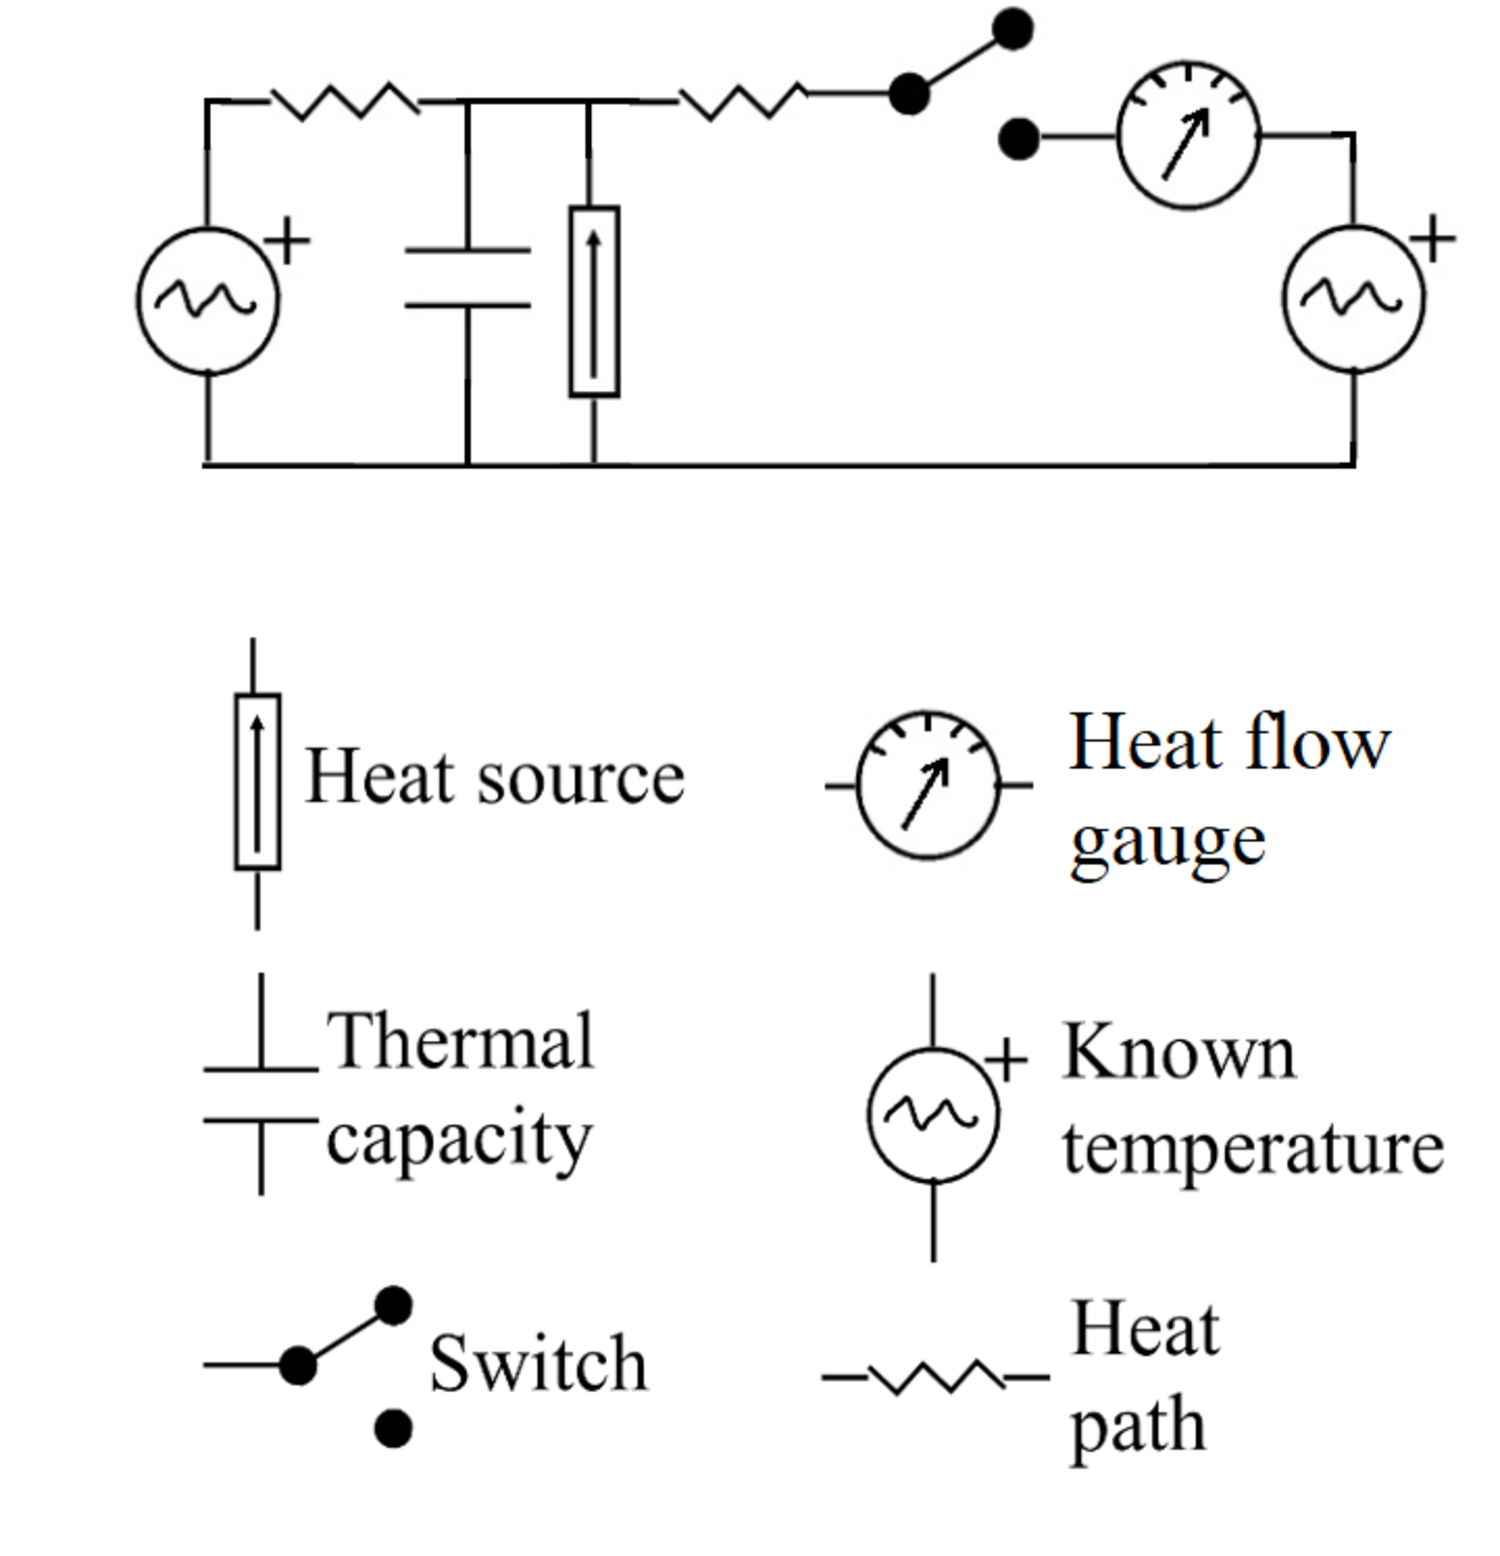
\includegraphics[width=4.5cm,height=4.5cm,keepaspectratio]{./pics/figAlf.pdf}}
\caption{xxxt}\vspace*{-6pt}
  \label{fig:alf}
\end{figure}

The conditioning system is governed in our case by a thermostat with a timer that turns it on and off. For this reason one need to consider that the RC-network that represents the phenomenon needs to change topologies depending on the operation (on or off) it is for this reason that we have considered a dual-mode RC-network as the one shown in Fig. \ref{fig:alf} and previously introduced by Ramallo-González on \citep{ramalloidentifying}.




Once the system was defined, an optimisation algorithm was used to find the values that minimise the RMSE (10 minutes intervals) of the simulated power consumption. To ensure that the data was used adequately, the total electricity consumption was separated onto an un-seasonal component and a seasonal one. The un-seasonal component was used as electric loads and the seasonal component was considered as the heating and cooling load. The building is equipped with a boiler and radiators network (???) that contribute to some of the heating loads. To take into account this effect, the outside temperature on the heating season was risen to a value in which the cooling and heating loads of the building were compensated.

The optimisation method to find the parameters of the model was a simplex. The termination criteria was to get a change on the solution smaller than 0.01 in all parameters. The calculation took approximately 6 minutes on a i5 Intel computer 2.7 running single threaded.





\subsection{Model Accuracy Metrics}

To assess model accuracy, this work uses two metrics: the mean absolute percentage of error (MAPE) and the coefficient of variation of the room mean squared error (CVRMSE).
The MAPE metric has been used in a wide number of electricity prediction studies \cite{fan2014development, edwards2012predicting}
. It expresses the average absolute error as a percentage and is calculated as follows:

\[
 MAPE = \frac{1}{n}\sum_{i=1}^{n} \frac{|y_i-\bar{y_i}|}{y_i}\times 100,
\]

where $y_i$ is the real consumption, $\bar{y_i}$ is the predicted consumption and $n$ is the number of observations.

Whereas the CVRMSE has often been used in energy prediction studies \citep{quilumba2015using} %26
. It evaluates how much error varies with respect
to the actual consumption mean and is calculated as follows:

\[
 CVRMSE = \frac{\sqrt{\frac{1}{n-1}\sum_{i=1}^{n}(y_i-\bar{y_i})^2}}{\bar{y}} \times 100,
\]


\subsection{Savings Metrics}

To determine energy savings and uncertainty levels from energy efficiency measures, the IPMVP [13] and ASHRAE’s Guideline 14 [2] provide three methods. The one that is suitable for our approach is whole-building metering, since it compares the total energy demand or cost during pre-experiment and post-experiments periods.

How to assess the accuracy and usefulness of whole-building energy models by testing predictions of baseline energy use against actual energy use being the objective to quantify and minimize the uncertainty in reported whole-building savings, which depends
on baseline model effectiveness, building predictability, and depth of savings being measured \cite{kramer2013energy}.

The predictive baseline models have as an output the metered pre-experiment energy use energy$_{pre}$ and uses the predictors such as environmental conditions inputs$_{pre}$ as inputs of the model. Therefore, the error in reported savings is proportional to the error in the baseline model forecasts.


\section{Use case}

The reference building in which the proposed procedure has been carried out to generate accurate building models is the Chemistry Faculty of the University of Murcia, which is a pilot building for the H2020 project ENTROPY \footnote{http://entropy-project.eu/}.  

The data that is used in order to build and train our baseline is 1 year data, from February 2016 to February 2017. 

\begin{figure}[h]%\vspace*{4pt}
\centering
\centerline{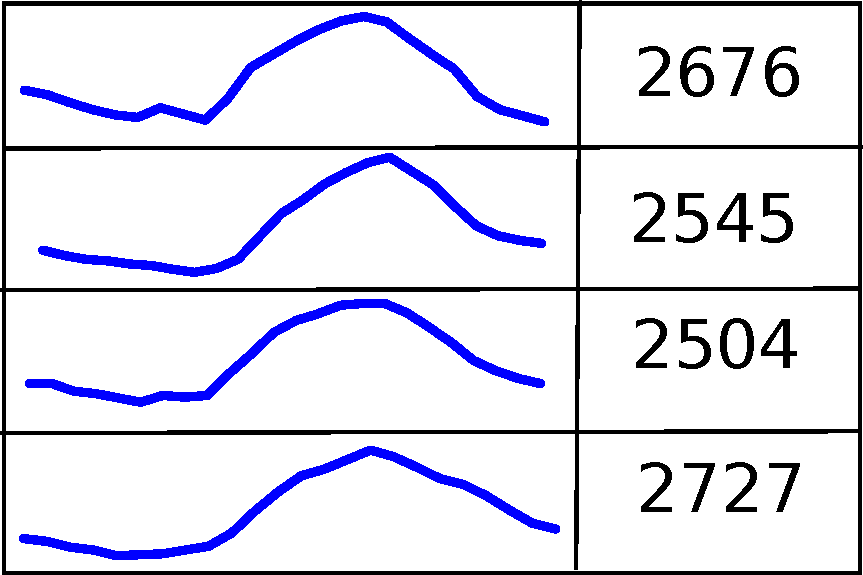
\includegraphics[width=4.5cm,height=4.5cm,keepaspectratio]{./pics/table_inputs_outputs.pdf}}
\caption{Daily temperature time series input and consumption output}\vspace*{-6pt}
  \label{fig:inout}
\end{figure}

\subsection{Black box approach}

Our black box methodology is highly versatile with respect to the input data, that is, it allows the addition of variables with minimal effort. In a constructive way, we start by relating the 24 temperature values of each day with the energy consumption of the building (see Fig. \ref{fig:inout}).

Having introduced the daily temperature time series, we consider that the addition of a categorical variable indicating season is irrelevant. However, the subject building has several features that are typical of educational buildings: the load %is temperature-dependent load 
on weekends is substantially lower than the load on weekdays and there are also differences between the day of the week (mainly Fridays).
In those terms, we use analysis of variance (ANOVA) in order to determine wether there exist differences between the consumption of the different days of the week (p-value = 0.001 $<$ 0.05) . 	In a posthoc test, the conclusion is that we can consider that Fridays have a different behaviour than the rest of the days, due to a disminishment on occupation. That way, we can add a dychotomus variable that indicates the kind of the of the week. Weekends and holidays consumption is estimated with the mean of the previous weekends and holidays.

\subsection{Grey box approach}

In the case of our grey box methodology, in order to avoid physically unrealistic results, the data was separated into heating and cooling periods. Any cooling on the heating season or vice versa was made zero.

Once the system was defined, an optimisation algorithm was used to find the values that minimise the RMSE (10 minutes intervals) of the simulated power consumption. To ensure that the data was used adequately, the total electricity consumption was separated onto an un-seasonal component and a seasonal one. The un-seasonal component was used as electric loads and the seasonal component was considered as the heating and cooling load. The building is equipped with a boiler and radiators network that contribute to some of the heating loads. To take into account this effect, the outside temperature on the heating season was risen to a value in which the cooling and heating loads of the building were compensated.
The optimisation method to find the parameters of the model was a simplex. The termination criteria was to get a change on the solution smaller than 0.01 in all parameters. %The calculation took approximately 6 minutes on a i5 Intel computer 2.7 running single threaded.

\subsection{Results}


\begin{center}
\begin{tabular}{cc|c|c|c|c}
\cline{3-5}
& & \multicolumn{3}{ c| }{Models} \\ \cline{3-5}
& & SVM & RF & XGB &  \\ \cline{1-5}
\multicolumn{1}{ |c  }{\multirow{2}{*}{Daily} } &
\multicolumn{1}{ |c| }{CVRMSE} & 12.4 & 9 & 11 &       \\ \cline{2-5}
\multicolumn{1}{ |c  }{}                        &
\multicolumn{1}{ |c| }{MAPE} & 7.2 & 6 & 7.3 &       \\ \cline{1-5}
\multicolumn{1}{ |c  }{\multirow{2}{*}{Weekly} } &
\multicolumn{1}{ |c| }{CVRMSE} & 6.4 & 5 & 6.2 &    \\ \cline{2-5}
\multicolumn{1}{ |c  }{}                        &
\multicolumn{1}{ |c| }{MAPE} & 5.2 & 4.5 & 5.5 &    \\ \cline{1-5}
\end{tabular}

\end{center}



\begin{figure}[h]%\vspace*{4pt}
\centering
\centerline{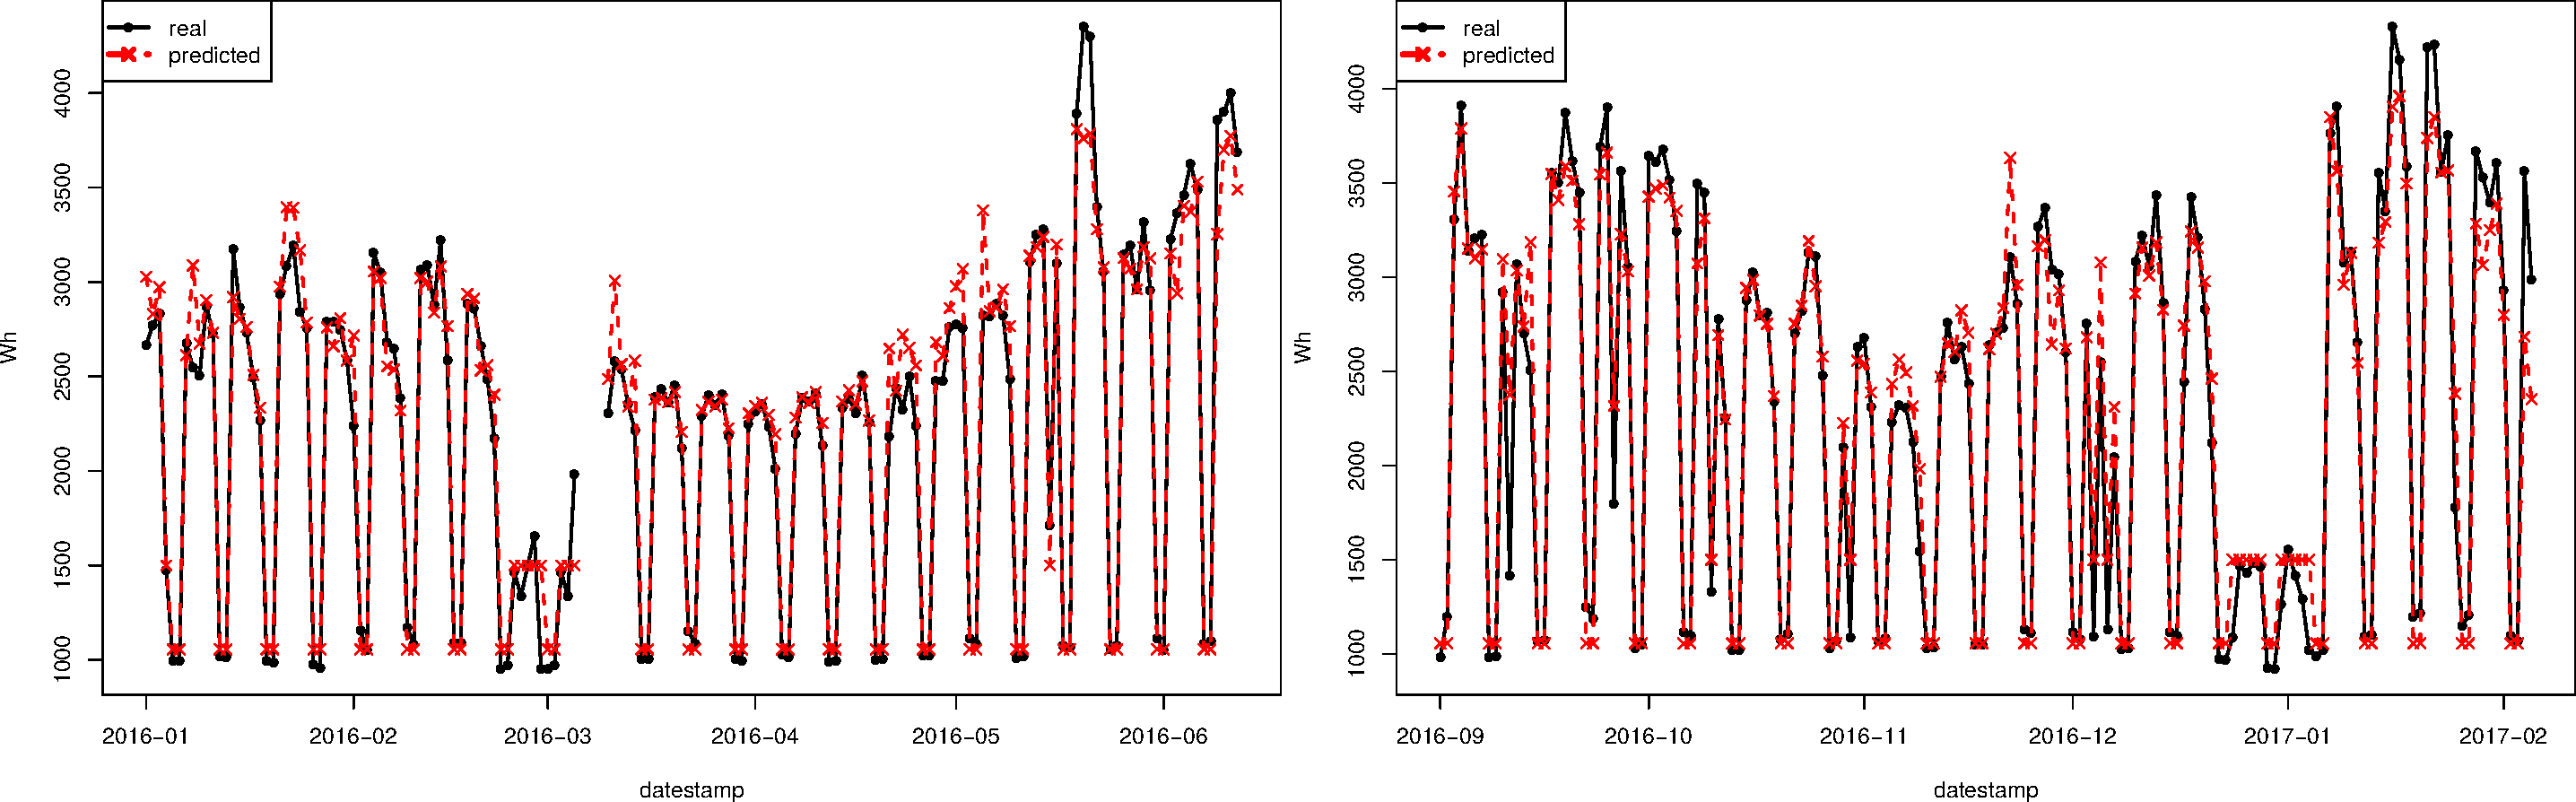
\includegraphics[width=15.5cm,height=15.5cm,keepaspectratio]{./pics/two_daily.pdf}}
\caption{Daily predictions using RF and real consumption}\vspace*{-6pt}
  \label{fig:daily}
\end{figure}

\begin{figure}[h]%\vspace*{4pt}
\centering
\centerline{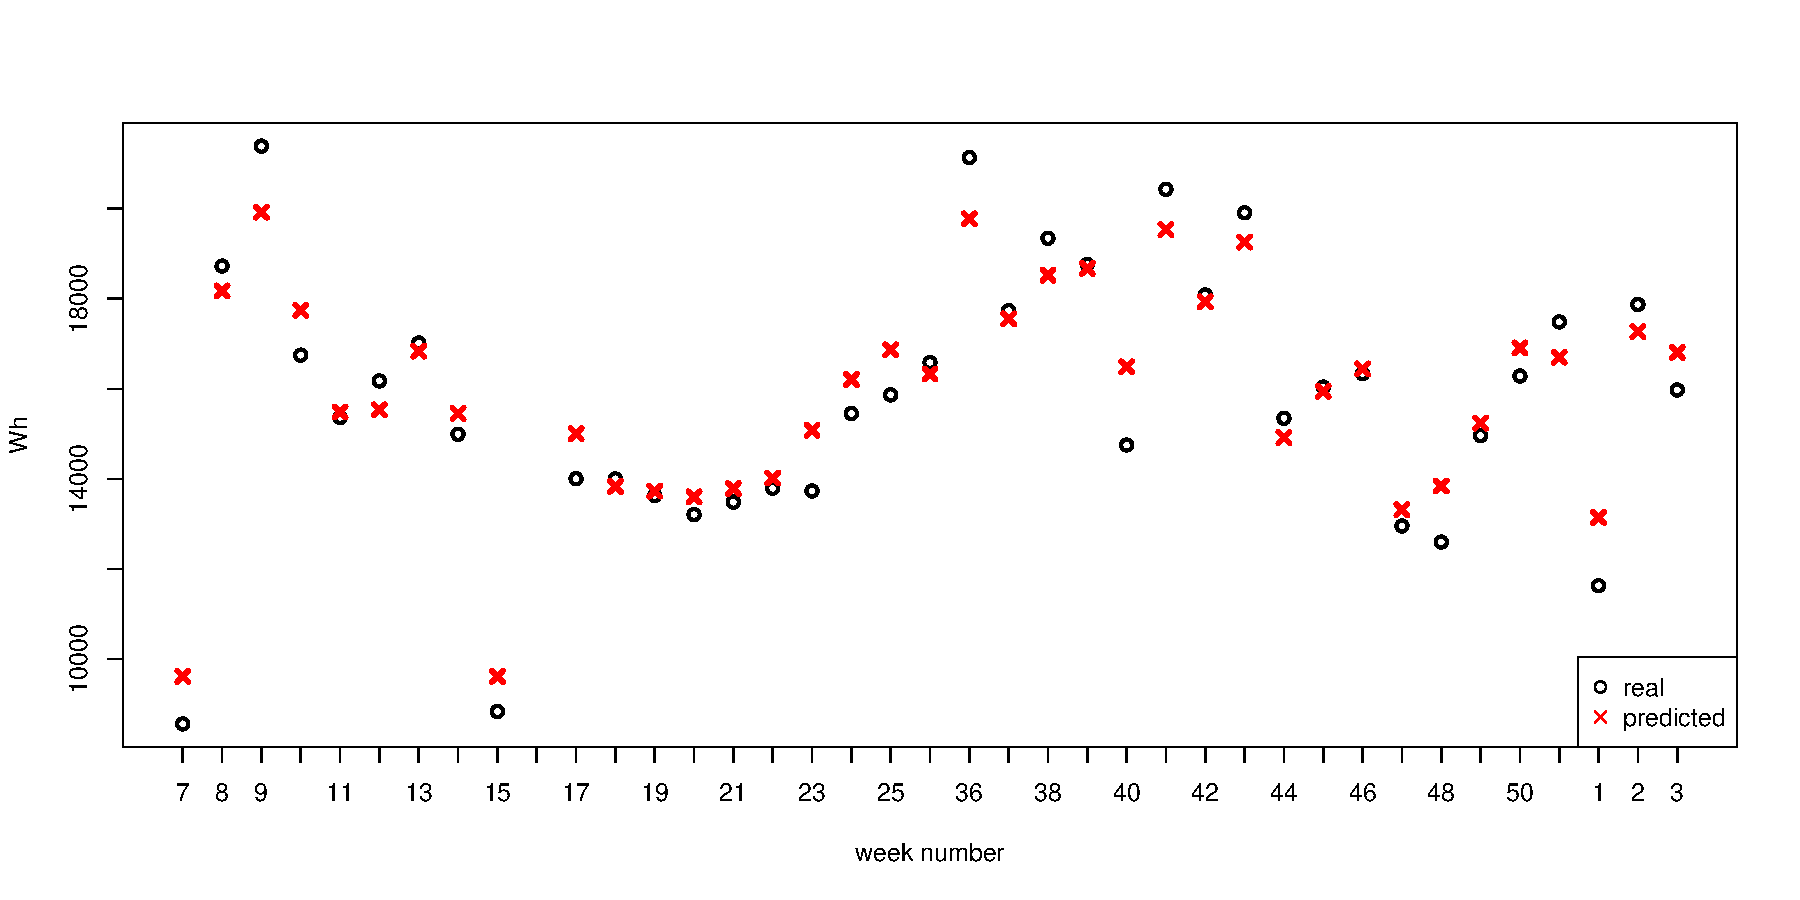
\includegraphics[width=12cm,height=12cm,keepaspectratio]{./pics/weekly_RF1.pdf}}
\caption{Weekly predictions using RF and real consumption}\vspace*{-6pt}
  \label{fig:weekly}
\end{figure}

\section{Discussion}




\section{Conclusions and future work}

This paper shows a study on

A very important characteristic of the black box approach is its generality. Even if we would have obtained similar results with the grey box models, they are clearly more generalizable than those. That way, a future via of research consists on the 

\section{Acknowledgements}

\bibliographystyle{elsarticle-num}

\bibliography{bib.bib}



\end{document}
modifications